\documentclass{article}
\usepackage[margin=1in]{geometry}
\usepackage{amsmath,amsthm,amssymb}
\usepackage{bbm,enumerate,mathtools}
\usepackage{tikz,pgfplots}
\usepackage{chessboard}
\usepackage[hidelinks]{hyperref}
\usepackage{multicol} % Problem 35

\newenvironment{question}{\begin{trivlist}\item[\textbf{Question.}]}{\end{trivlist}}
\newenvironment{note}{\begin{trivlist}\item[\textbf{Note.}]}{\end{trivlist}}
\newenvironment{references}{\begin{trivlist}\item[\textbf{References.}]}{\end{trivlist}}
\newenvironment{related}{\begin{trivlist}\item[\textbf{Related.}]\end{trivlist}\begin{enumerate}}{\end{enumerate}}


\begin{document}

\rating{3}{3}
According to Wikipedia
\begin{quote}
  A Johnson solid is a strictly convex polyhedron for which each face
  is a regular polygon.
\end{quote}
Let $\operatorname{Hull}(P)$ denote the convex hull of a polygon $P$.
Say that a $1$-concave Johnson solid is a polyhedra $P$ with regular polygonal
faces (such that no two faces lay the same plane) and with the property that the
``concave'' part $\operatorname{Hull}(P) - P$ is a connected convex polyhedron.

\begin{figure}[ht!]
  \centering
  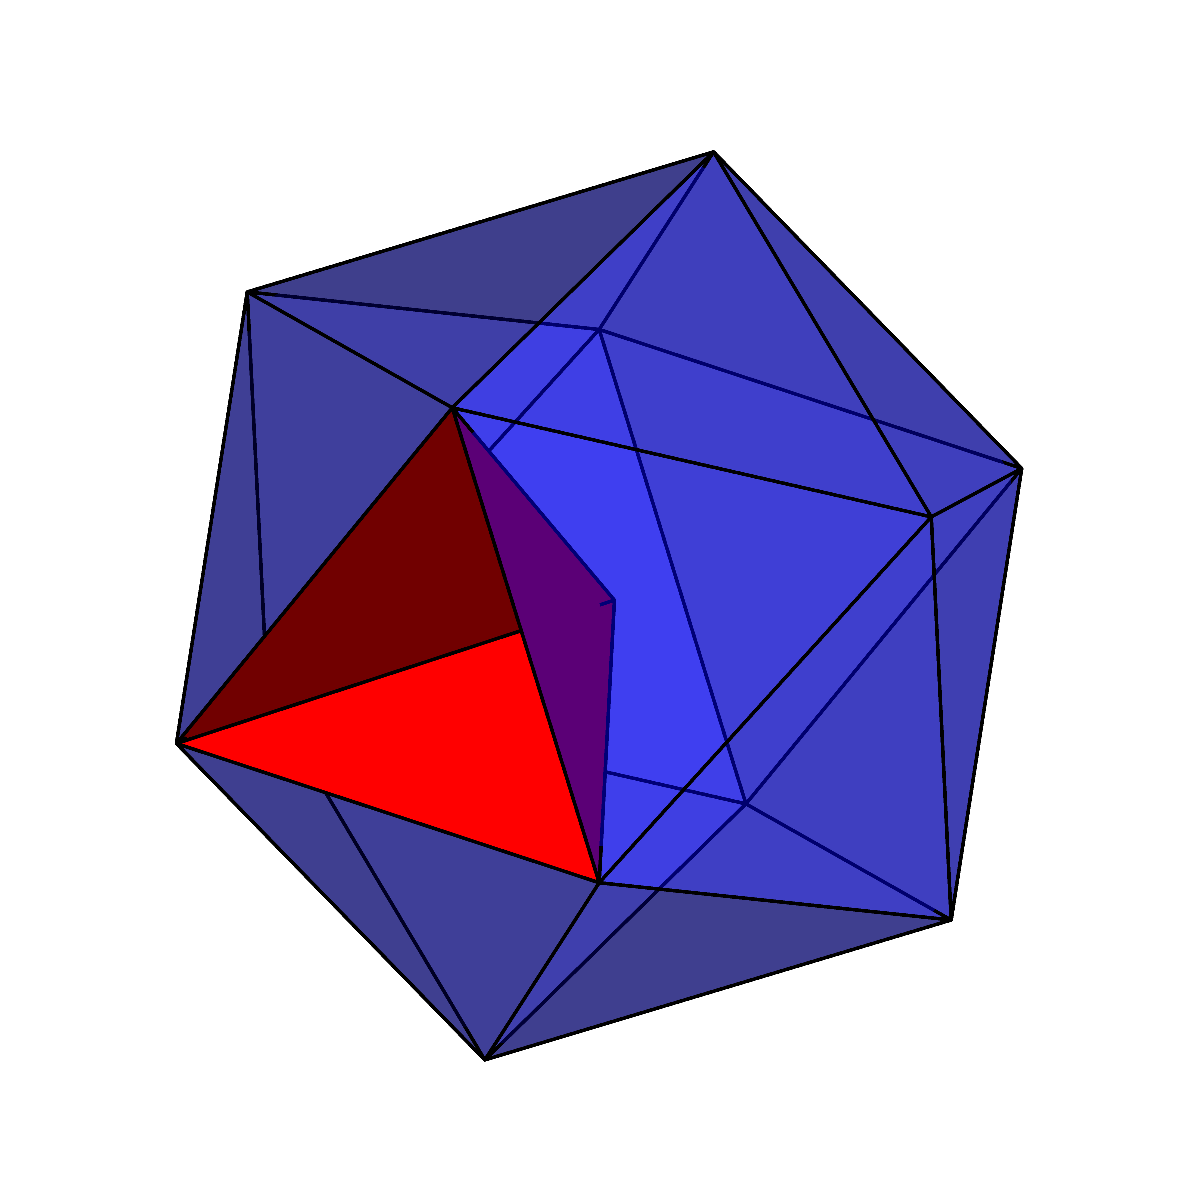
\includegraphics[scale=0.18]{assets/114_problem/icosahedron-tetrahedron_side_view.png}
  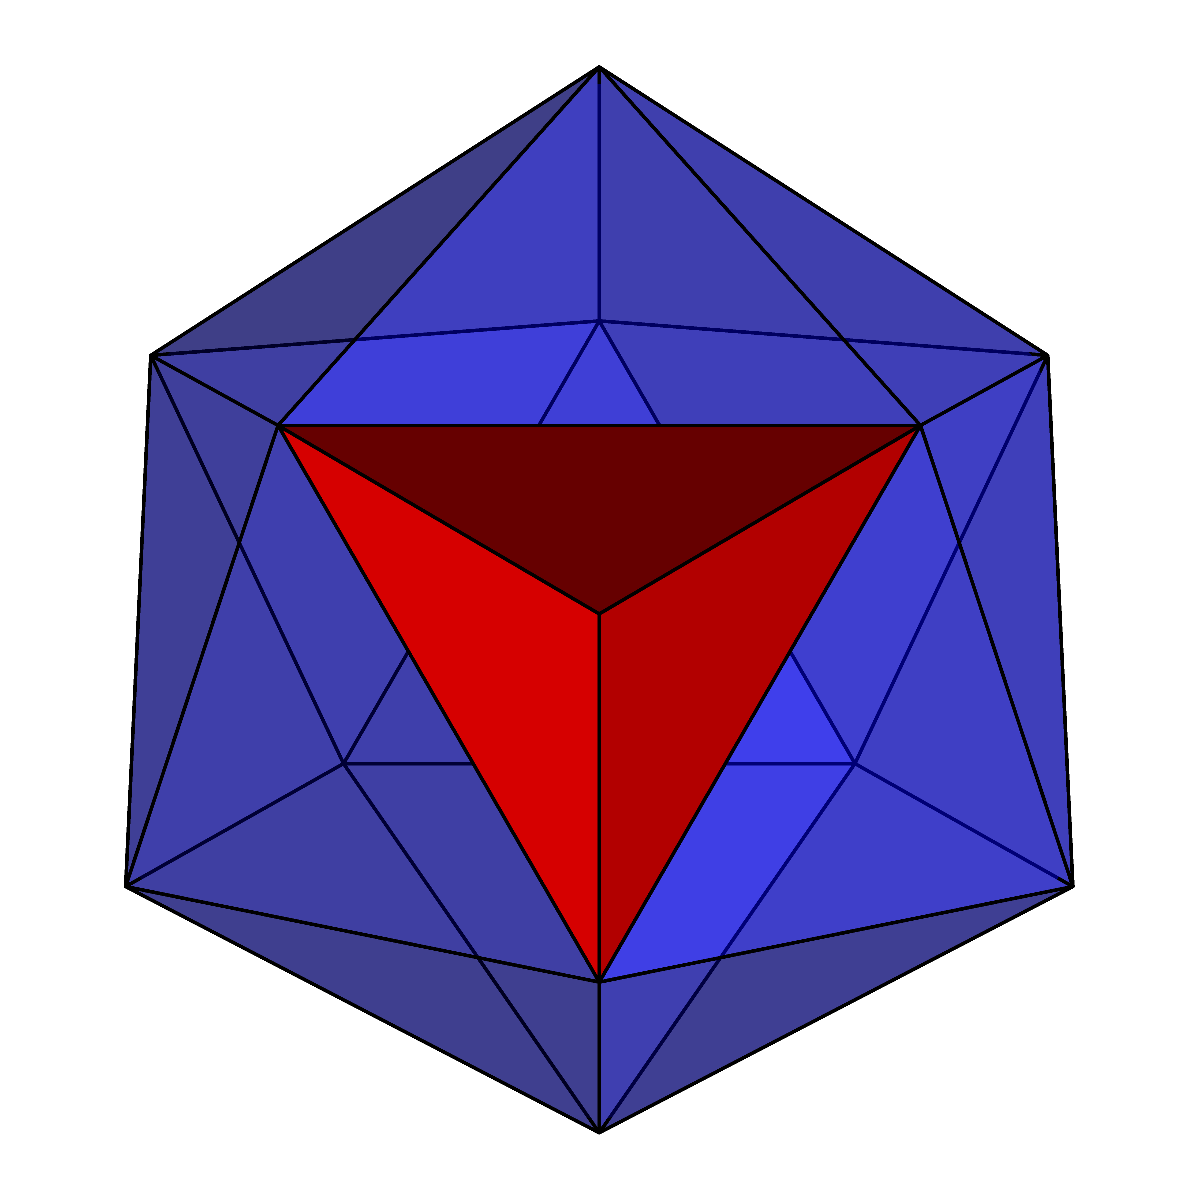
\includegraphics[scale=0.18]{assets/114_problem/icosahedron-tetrahedron_top_view.png}
  \caption{An example of a ``$1$-concave'' Johnson solid: an icosahedron with a tetrahedron removed.}
\end{figure}

\begin{question}
  Excluding infinite families of $1$-concave Johnson solids
  (e.g. prisms with a square pyramid removed),
  are there a finite number of $1$-concave Johnson solids?
\end{question}

\begin{related}
  \item What if the ``co-planar'' restriction is relaxes so that no two
    \textit{adjacent} faces may lie in the same plane?
  \item How many $1$-concave Johnson solids have a convex hull that is a
    Johnson solid?
  \item Say that a $2$-concave Johnson solid $P$ is a polyhedra with regular
    polygonal faces such that
    $P' = \operatorname{Hull}(P) - P$ is a connected polyhedron, and
    $\operatorname{Hull}(P') - P'$ is a connected convex polyhedron.
    Outside of infinite families,
    are there a finite number of $2$-concave Johnson solids?
    $n$-concave Johnson solids?
  \item Are all $n$-concave Johnson solids homeomorphic to a sphere?
  \item Do there exist $k$-concave Johnson solids for all $k$?
\end{related}

\begin{references}
  \item Problem 53.
  \item \url{https://en.wikipedia.org/wiki/Johnson_solid}
\end{references}
\end{document}

% Mathematica code for images.
% IcosahedronCoordinates := PolyhedronData["Icosahedron", "VertexCoordinates"];
% PerpV := Cross[
%   IcosahedronCoordinates[[1]] - IcosahedronCoordinates[[6]],
%   IcosahedronCoordinates[[1]] - IcosahedronCoordinates[[5]]
% ];
% UnitV := PerpV/Norm[PerpV];
% TCenter := RegionCentroid[Triangle[{
%   IcosahedronCoordinates[[1]],
%   IcosahedronCoordinates[[5]],
%   IcosahedronCoordinates[[6]]
% }]];
% TetrahedronCoordinate = TCenter - (Sqrt[6]/3)*UnitV;
% ViewFrom[c_] := Graphics3D[{
%   EdgeForm[{Thickness[0.003], Black}],
%   Red,
%   Polyhedron[
%    Append[IcosahedronCoordinates, TetrahedronCoordinate], {
%     {1, 5, 13}, {1, 6, 13}, {5, 6, 13}
%     }
%   ],
%   Blue, Opacity[0.5],
%   Polyhedron[IcosahedronCoordinates, {
%     {1, 5, 9}, {1, 9, 3}, {1, 3, 10}, {1, 10, 6},
%     {2, 7, 11}, {2, 11, 4}, {2, 4, 12}, {2, 12, 8}, {2, 8, 7},
%     {7, 8, 3}, {8, 12, 10}, {12, 4, 6}, {4, 11, 5}, {11, 7, 9},
%     {6, 10, 12}, {10, 3, 8}, {3, 9, 7}, {9, 5, 11}, {5, 6, 4}
%   }]
% },
%   ViewVertical -> {0, 0, 1},
%   ViewVector -> {c, {0, 0, 0}},
%   Boxed -> False
% ]
% Export["Desktop/TopView.png", ViewFrom[{4.0, 0, -5.3}],
%  ImageSize -> 1200, "CompressionLevel" -> 0]
% Export["Desktop/SideView.png", ViewFrom[200*{2, 3, -5}],
%  ImageSize -> 1200, "CompressionLevel" -> 0]
